% questions.tex —— 2008 年·普通高等学校招生考试·四川卷·文科 · 题目内容片段（无答案）
% 由 tools/generate_projects.py 依来源总账自 2008/2008_数学真题_四川文_试题.md 生成，勿手改（改源 MD 后重跑）


\gkpart{一、选择题}

\begin{question}
\gkti{1}设集合 $U=\{1,2,3,4,5\}$，$A=\{1,2,3\}$，$B=\{2,3,4\}$，则 $\complement_U(A\cap B)=$（　）

（A）$\{2,3\}$

（B）$\{1,4,5\}$

（C）$\{4,5\}$

（D）$\{1,5\}$

\end{question}
\begin{question}
\gkti{2}函数 $y=\ln(2x+1)$（$x>-\dfrac12$）的反函数是（　）

（A）$y=\dfrac12\mathrm e^x-1$（$x\in\mathbf R$）

（B）$y=\mathrm e^{2x}-1$（$x\in\mathbf R$）

（C）$y=\dfrac12(\mathrm e^x-1)$（$x\in\mathbf R$）

（D）$y=\mathrm e^{\frac x2}-1$（$x\in\mathbf R$）

\end{question}
\begin{question}
\gkti{3}设平面向量 $\boldsymbol a=(3,5)$，$\boldsymbol b=(-2,1)$，则 $\boldsymbol a-2\boldsymbol b=$（　）

（A）$(7,3)$

（B）$(7,7)$

（C）$(1,7)$

（D）$(1,3)$

\end{question}
\begin{question}
\gkti{4}$(\tan x+\cot x)\cos^2x=$（　）

（A）$\tan x$

（B）$\sin x$

（C）$\cos x$

（D）$\cot x$

\end{question}
\begin{question}
\gkti{5}不等式 $|x^2-x|<2$ 的解集为（　）

（A）$(-1,2)$

（B）$(-1,1)$

（C）$(-2,1)$

（D）$(-2,2)$

\end{question}
\begin{question}
\gkti{6}直线 $y=3x$ 绕原点逆时针旋转 $90^\circ$，再向右平移 $1$ 个单位，所得到的直线为（　）

（A）$y=-\dfrac13x+\dfrac13$

（B）$y=-\dfrac13x+1$

（C）$y=3x-3$

（D）$y=3x+1$

\end{question}
\begin{question}
\gkti{7}$\triangle ABC$ 的三个内角 $A$、$B$、$C$ 的对边边长分别是 $a$、$b$、$c$。若 $a=\dfrac{\sqrt5}2b$，$A=2B$，则 $\cos B=$（　）

（A）$\dfrac{\sqrt5}3$

（B）$\dfrac{\sqrt5}4$

（C）$\dfrac{\sqrt5}5$

（D）$\dfrac{\sqrt5}6$

\end{question}
\begin{question}
\gkti{8}设 $M$ 是球 $O$ 的半径 $OP$ 的中点，分别过 $M$、$O$ 作垂直于 $OP$ 的平面，截球面得到两个圆，则这两个圆的面积比值为（　）

（A）$\dfrac14$

（B）$\dfrac12$

（C）$\dfrac23$

（D）$\dfrac34$

\end{question}
\begin{question}
\gkti{9}设定义在 $\mathbf R$ 上的函数 $f(x)$ 满足 $f(x)\cdot f(x+2)=13$，若 $f(1)=2$，则 $f(99)=$（　）

（A）$13$

（B）$2$

（C）$\dfrac{13}2$

（D）$\dfrac2{13}$

\end{question}
\begin{question}
\gkti{10}设直线 $l\subset$ 平面 $\alpha$，过平面 $\alpha$ 外一点 $A$ 与 $l$、$\alpha$ 都成 $30^\circ$ 角的直线有且只有（　）

（A）$1$ 条

（B）$2$ 条

（C）$3$ 条

（D）$4$ 条

\end{question}
\begin{question}
\gkti{11}已知双曲线 $C:\dfrac{x^2}9-\dfrac{y^2}{16}=1$ 的左、右焦点分别为 $F_1$、$F_2$，$P$ 为 $C$ 的右支上一点，且 $|PF_2|=|F_1F_2|$，则 $\triangle PF_1F_2$ 的面积等于（　）

（A）$24$

（B）$36$

（C）$48$

（D）$96$

\end{question}
\begin{question}
\gkti{12}若三棱柱的一个侧面是边长为 $2$ 的正方形，另外两个侧面都是有一个内角为 $60^\circ$ 的菱形，则该棱柱的体积为（　）

（A）$\sqrt2$

（B）$2\sqrt2$

（C）$3\sqrt2$

（D）$4\sqrt2$

\end{question}
\gkpart{二、填空题}

\begin{question}
\gkti{13}$(1+2x)^3(1-x)^4$ 展开式中 $x$ 的系数为\gkblank{}。

\end{question}
\begin{question}
\gkti{14}已知直线 $l:x-y+4=0$ 与圆 $C:(x-1)^2+(y-1)^2=2$，则 $C$ 上各点到 $l$ 的距离的最小值为\gkblank{}。

\end{question}
\begin{question}
\gkti{15}从甲、乙等 $10$ 名同学中挑选 $4$ 名参加某项公益活动，要求甲、乙中至少有 $1$ 人参加，则不同的挑选方法有\gkblank{}种。

\end{question}
\begin{question}
\gkti{16}设数列 $\{a_n\}$ 中，$a_1=2$，$a_{n+1}=a_n+n+1$，则通项 $a_n=$\gkblank{}。

\end{question}
\gkpart{三、解答题}

\begin{question}
\gkti{17}求函数 $y=7-4\sin x\cos x+4\cos^2x-4\cos^4x$ 的最大值与最小值。

\end{question}
\begin{question}
\gkti{18}设进入某商场的每一位顾客购买甲种商品的概率为 $0.5$，购买乙种商品的概率为 $0.6$，且购买甲种商品与购买乙种商品相互独立，各顾客之间购买商品是相互独立的。

（1）求进入商场的 $1$ 位顾客购买甲、乙两种商品中的一种的概率；

（2）求进入该商场的 $3$ 位顾客中，至少有 $2$ 位顾客既未购买甲种也未购买乙种商品的概率。

\Needspace{0.4\textheight}
\end{question}
\begin{question}
\gkti{19}如图，平面 $ABEF\perp$ 平面 $ABCD$，四边形 $ABEF$ 与 $ABCD$ 都是直角梯形，$\angle BAD=\angle FAB=90^\circ$，$BC\parallel\dfrac12AD$，$BE\parallel\dfrac12AF$，$G$、$H$ 分别是 $FA$、$FD$ 的中点。

（1）证明：四边形 $BCHG$ 是平行四边形；

（2）$C$、$D$、$E$、$F$ 四点是否共面？为什么？

（3）设 $AB=BE$。证明：平面 $ADE\perp$ 平面 $CDE$。
\nopagebreak[4]
\begin{center}% 2008 年四川卷文科第 19 题：平面 ABEF ⊥ 平面 ABCD，两个直角梯形 ABEF、ABCD，
%   ∠BAD = ∠FAB = 90°，BC ∥= ½AD，BE ∥= ½AF，G、H 为 FA、FD 中点。
% 来源 PDF：gaokaomath-src/普通高考/2008/2008四川文.pdf
% SHA-256：1ba08ce1f61bedd8f036654d1054bebc1fda2ff655e05813ee4a45c552cc9c3e
% 原页：2008四川文.pdf 第 2 页（A3 三栏）第 1 栏，书页码 486。
% 绘图方式：按直角坐标建系后作斜投影 (x,y,z) -> (x+0.8y, 0.5y+z)，再整体缩放。
%   取 A(0,0,0)、B(2,0,0)、C(2,2,0)、D(0,4,0)、F(0,0,4)、E(2,0,2)，
%   则 G(0,0,2)、H(0,2,2)；底面 ABCD 的 AD、AC 与体对角线 AE、GH 用虚线。
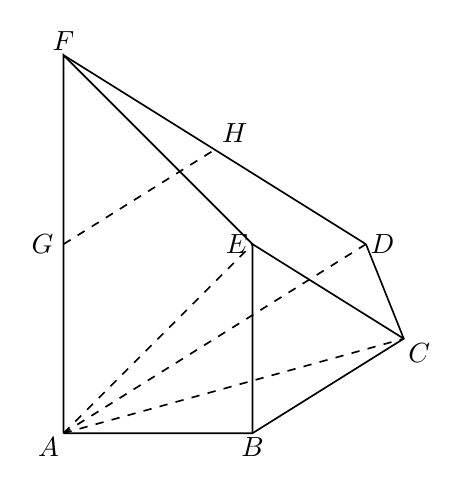
\begin{tikzpicture}[scale=1.2, semithick, every node/.style={inner sep=1.4pt}]
  \coordinate (A) at (0.00,0.00);
  \coordinate (B) at (2.00,0.00);
  \coordinate (C) at (3.60,1.00);
  \coordinate (D) at (3.20,2.00);
  \coordinate (F) at (0.00,4.00);
  \coordinate (E) at (2.00,2.00);
  \coordinate (G) at (0.00,2.00);
  \coordinate (H) at (1.60,3.00);

  % 底面 ABCD
  \draw (A) -- (B) -- (C) -- (D);
  \draw[dashed] (D) -- (A);
  \draw[dashed] (A) -- (C);

  % 立面 ABEF
  \draw (A) -- (F) -- (E) -- (B);

  % 侧棱与内部虚线
  \draw (C) -- (E);
  \draw (D) -- (F);
  \draw[dashed] (A) -- (E);
  \draw[dashed] (G) -- (H);

  \node[below left] at (A) {$A$};
  \node[below] at (B) {$B$};
  \node[below right] at (C) {$C$};
  \node[right] at (D) {$D$};
  \node[above] at (F) {$F$};
  \node[left] at (E) {$E$};
  \node[left=2pt] at (G) {$G$};
  \node[above right=1pt] at (H) {$H$};
\end{tikzpicture}
\end{center}
\nopagebreak[4]
\end{question}
\begin{question}
\gkti{20}设 $x=1$ 和 $x=2$ 是函数 $f(x)=x^5+ax^3+bx+1$ 的两个极值点。

（1）求 $a$ 和 $b$ 的值；

（2）求 $f(x)$ 的单调区间。

\end{question}
\begin{question}
\gkti{21}已知数列 $\{a_n\}$ 的前 $n$ 项和 $S_n=2a_n-2^n$。

（1）求 $a_3$，$a_4$；

（2）证明：数列 $\{a_{n+1}-2a_n\}$ 是等比数列；

（3）求 $\{a_n\}$ 的通项公式。

\end{question}
\begin{question}
\gkti{22}设椭圆 $\dfrac{x^2}{a^2}+\dfrac{y^2}{b^2}=1$（$a>b>0$）的左、右焦点分别为 $F_1$、$F_2$，离心率 $e=\dfrac{\sqrt2}2$，点 $F_2$ 到右准线 $l$ 的距离为 $\sqrt2$。

（1）求 $a$、$b$ 的值；

（2）设 $M$、$N$ 是右准线 $l$ 上两个动点，满足 $\overrightarrow{F_1M}\cdot\overrightarrow{F_2M}=0$。证明：当 $|MN|$ 取最小值时，$\overrightarrow{F_2F_1}+\overrightarrow{F_2M}+\overrightarrow{F_2N}=\boldsymbol 0$。

\end{question}